\section{A joining cost with one entropy budget}
\label{canonical:section}

The energy decomposition \eqref{main:energy-split} leaves the cost of
joining the two faces of a coordinate split. We minimize this cost at
fixed child means and average conditional entropy. Allowing arbitrary
coupled pair laws is a valid relaxation because only a lower bound on
the actual joining cost is needed; no independence of the faces is assumed.
The symmetric fixed-entropy problem of
Chen--Gohari--Nair \cite[Theorem~4 and Section~IV-C]{ChenGohariNair2025}
has an optimizer supported on a reflected interior pair and the two
equal-output corners. Chen et al.\ \cite[Section~3.1, Theorem~3.10]{ChenEtAl2026CK}
characterize related three-point optimizers when both means and both
entropy moments are prescribed, under explicit contact and mass conditions.
Here we prescribe the two means but constrain only the average entropy.
Pricing this common entropy budget gives the optimizer throughout the
domain, including the transition from two corners to one.

For interior $x,y$, use the joining cost
\begin{equation}
 c(x,y)=\frac{x-y}{4}\,[V(x)-V(y)].
 \label{canonical:cost}
\end{equation}
It is symmetric and nonnegative.  Extend it by zero at the equal
corners $(1,1),(-1,-1)$ and by $+\infty$ at every other boundary pair.
This is a lower semicontinuous, jointly convex function.  Indeed,
\[
 c(x,y)=\frac18\{J(1+x,1+y)+J(1-x,1-y)\},
 \qquad J(s,t)=(s-t)\log(s/t),
\]
and $J$ is the sum of two relative-entropy perspectives.

Fix $-1<b<a<1$, and write
\[
 m=\frac{a+b}{2},\qquad \delta=\frac{a-b}{2},\qquad
 e_{\max}=\frac{H(a)+H(b)}2.
\]
Jensen's inequality makes $e_{\max}$ the largest possible average
entropy; the deterministic pair attains it.  We call this boundary
the capacity state of the joining problem.
For $0<e\le e_{\max}$, define
\begin{equation}
 \mathcal K(m,\delta,e)=
 \inf\left\{\E c(A,B):
 \E A=a,\ \E B=b,\
 \frac{\E H(A)+\E H(B)}2\le e\right\}.
 \label{canonical:budget}
\end{equation}
The infimum is over joint laws on $[-1,1]^2$.  Only the average entropy
is constrained.

\subsection{Constructing and certifying the priced core}

We first construct candidate laws of the form
\begin{equation}
 \lambda\delta_{(x,y)}
 +\pi_+\delta_{(1,1)}+\pi_-\delta_{(-1,-1)},\qquad -1<y<x<1.
 \label{canonical:law}
\end{equation}
The prescribed mean difference forces $\lambda(x-y)=2\delta$;
the mean sum and total mass then determine the two corner masses.
We will minimize a priced objective within this family, and then
prove optimality against all coupled laws by an affine lower bound.

For an ordered interior pair $x>y$, set
\[
 z=\log\frac{1+x}{1+y},\quad
 w=\log\frac{1-y}{1-x},\quad
 u=(e^z-1)^{-1},\quad v=(e^w-1)^{-1},\quad n=1+u+v.
\]
Then
\begin{equation}
 x=\frac{1+u-v}{n},\qquad
 y=\frac{u-v-1}{n},\qquad x-y=\frac2n,\qquad
 \frac{c(x,y)}{x-y}=\frac{z+w}{8}.
 \label{canonical:coordinates}
\end{equation}
In these coordinates, the masses required by the two means are
\begin{equation}
 \lambda=\delta n,\qquad
 \pi_+=\frac{1+b-2\delta u}{2},\qquad
 \pi_-=\frac{1-a-2\delta v}{2}.
 \label{canonical:masses}
\end{equation}
They sum to one, and the corner masses are nonnegative exactly when
\begin{equation}
 z\ge z_0:=\log\frac{1+a}{1+b},\qquad
 w\ge w_0:=\log\frac{1-b}{1-a}.
 \label{canonical:floors}
\end{equation}
For a price $p\ge0$, define
\[
 \mathcal H(z,w)=\frac{H(x)+H(y)}{x-y},\qquad
 F_p(z,w)=\frac{z+w}{8}+p\mathcal H(z,w).
\]
The corners contribute neither cost nor entropy. Hence the priced
objective of the candidate law \eqref{canonical:law} is
\begin{equation}
 \E\{c(A,B)+p[H(A)+H(B)]\}=2\delta F_p(z,w).
 \label{canonical:candidate-value}
\end{equation}
This explains the normalization by $x-y$: the prescribed mean
difference absorbs the core mass. The remaining task is to minimize
$F_p$ subject to \eqref{canonical:floors} and certify that its value
also bounds every other pair law.

The normalized entropy has the positive series
\begin{equation}
\begin{split}
 \mathcal H(z,w)
 &=\frac{q(z)+q(w)}2+
 \sum_{i,j\ge1}\frac{e^{-iz-jw}}{\max(i,j)},\\
 q(t)&=\frac{t}{e^t-1}-\log(1-e^{-t}).
\end{split}
 \label{canonical:entropy-series}
\end{equation}
Here is a direct verification.  The normalized entropy of $x$ is
$[n\log n-(u+1)\log(u+1)-v\log v]/2$, and that of $y$ is its
transpose.  Put $\xi=e^{-z}$ and $\zeta=e^{-w}$.  After subtracting
$[q(z)+q(w)]/2$, the sum becomes
\[
 n\log(1-\xi\zeta)-v\log(1-\xi)-u\log(1-\zeta).
\]
The coefficient of $\xi^i\zeta^j$ is
$1/i+1/j-1/\min(i,j)=1/\max(i,j)$, which proves
\eqref{canonical:entropy-series}.  The series and its derivatives
converge uniformly on compact subsets of the positive quadrant.

The function $\mathcal H$ is symmetric and strictly convex.  In fact,
with $v_t=(e^t-1)^{-1}$,
\[
 q''(t)=v_t(v_t+1)\{t(2v_t+1)-1\}>0,
\]
because $t(2v_t+1)=t\coth(t/2)>2$.  Each term in the double series
is convex; its exponential direction vectors span the plane.

\begin{lemma}[The priced core]
\label{canonical:priced}
For every $p\ge0$, the minimum of
\[
 \E\{c(A,B)+p[H(A)+H(B)]\},
 \qquad \E A=a,\quad \E B=b,
\]
has a unique optimizer.  It is one ordered interior pair $(x,y)$
and possible equal corners, as in \eqref{canonical:law}. Its core is
given by the unique minimizer of $F_p$ subject to
\eqref{canonical:floors}, using \eqref{canonical:coordinates};
its masses are \eqref{canonical:masses}.
At $p=0$, the optimizer is the deterministic pair $(a,b)$.
\end{lemma}

\begin{proof}
For $p>0$, strict convexity and the linear term give a unique
minimizer on the floored quadrant.  At $p=0$, the unique minimum is
$(z_0,w_0)$. We now turn this constrained minimum into an affine
lower bound in the pair values, valid for every coupled law.
At the selected point put
\[
 \gamma_+=\frac{(F_p)_z}{2u(u+1)},\qquad
 \gamma_-=\frac{(F_p)_w}{2v(v+1)}.
\]
Both are nonnegative; a derivative vanishes unless its floor is active.
The function
\[
 \mathscr Q(z,w)=F_p(z,w)+\gamma_+(1+2u)+\gamma_-(1+2v)
\]
has zero gradient at the selected point and is strictly convex on the
whole positive quadrant.  At $p=0$, both added coefficients are
positive, and $u''=u(u+1)(2u+1)>0$, with the same identity for $v$,
so strict convexity still holds. Let $\kappa>0$ be its minimum;
positivity follows from the positive linear term in $F_p$ and the
nonnegative remaining terms.  Multiplying $\mathscr Q\ge\kappa$ by $x-y$ gives the
global support
\begin{equation}
\begin{split}
 c(x,y)+p[H(x)+H(y)]-\kappa(x-y)
 +\gamma_+(2+x+y)+\gamma_-(2-x-y)\ge0.
\end{split}
 \label{canonical:support}
\end{equation}
For $x>y$ this is the convex minimum just proved.  For $x<y$, every
term is nonnegative and $-\kappa(x-y)>0$.  On the interior diagonal,
the entropy term is positive if $p>0$; if $p=0$, both corner
coefficients are positive.  At the equal corners, equality is allowed
exactly when the corresponding $\gamma$ vanishes.  All other boundary
pairs have infinite cost.

The candidate masses in \eqref{canonical:masses} have means $a,b$,
and complementarity gives $\gamma_\pm\pi_\pm=0$.
Thus \eqref{canonical:law} is supported at equality points of
\eqref{canonical:support}.  Averaging the support proves optimality.
Its only possible interior contact is the unique convex minimizer;
the mean difference fixes its mass, and the mean sum fixes the two
corners.  This proves uniqueness.
\end{proof}

\begin{proposition}[Exact entropy coverage]
\label{canonical:coverage}
For every $0<e\le e_{\max}$, a law of the form
\eqref{canonical:law} attains \eqref{canonical:budget} and has
average entropy exactly $e$.
\end{proposition}

\begin{proof}
Let $e(p)$ be the average entropy of the unique priced optimizer.
It is continuous for $p\ge0$: on each bounded price interval the
minimizers lie in a common compact subset of the floored quadrant,
since $F_p\ge(z+w)/8$; uniqueness then gives continuity.
Also $e(0)=e_{\max}$.

There are finite-cost laws with the prescribed means and arbitrarily
small entropy.  Choose a reflected core $(r,-r)$ with $r$ sufficiently
close to one, mass $\delta/r$, and the two equal-corner masses needed
to match $m$.  They are nonnegative because
$\delta<1-|m|$.  Its entropy $(\delta/r)H(r)$ tends to zero.
If such a comparison law has cost $C_\varepsilon$ and entropy at most
$\varepsilon$, priced optimality and nonnegativity of cost imply
\[
 2p\,e(p)\le C_\varepsilon+2p\varepsilon.
\]
Hence $e(p)\to0$ as $p\to\infty$.  Continuity supplies a price with
$e(p)=e$.

For any competing law whose average entropy $\widetilde e$ is at
most $e$, the global priced support gives
\[
 \E c(A,B)+2p\widetilde e
 \ge \E c(A_p,B_p)+2pe.
\]
Since $p\ge0$, its cost is at least that of the priced optimizer.
This proves the proposition without a signed entropy multiplier or
an abstract optimizer replacement.
\end{proof}

\subsection{The two canonical geometries}

By reflection assume $m\ge0$, so $z_0\le w_0$.  Symmetry and
uniqueness imply $z\le w$ at the priced minimizer: otherwise swapping
the coordinates is feasible and has the same value.
The case $p=0$ is already deterministic, so assume $p>0$ in the
following strict-convexity argument.
If $w>w_0$ and $z<w$, then $(F_p)_w=0$ while strict convexity and
symmetry give $(F_p)_z<(F_p)_w$, contradicting constrained
optimality.  Thus either $z=w$ or $w=w_0$.

In the first case, the core is $(r,-r)$, with
\begin{equation}
 k=\frac{\delta}{r},\qquad
 e=kH(r),\qquad
 \mathcal K=\delta V(r),\qquad 0\le m\le1-k.
 \label{canonical:reflected}
\end{equation}
At fixed $\delta,e$, the radius $r$ and the cost do not depend on
$m$.  Uniqueness of $r$ follows because $H(r)/r$ strictly decreases.

In the second case, $\pi_-=0$.  With core mass $k$,
\begin{equation}
\begin{split}
 1-m\le k\le1,\qquad
 x=1-\frac{1-a}{k},\quad y=1-\frac{1-b}{k},\\
 e=\frac{k}{2}[H(x)+H(y)],\qquad
 \mathcal K=k\,c(x,y).
\end{split}
 \label{canonical:onecorner}
\end{equation}
Indeed $z\le w$ means the core center is nonnegative, and
\[
 \frac{x+y}{2}=1-\frac{1-m}{k}\ge0.
\]
The two geometries meet at $k=1-m$, where the reflected core has
only a positive common corner.  Thus their entropy threshold is
\begin{equation}
 e_0(m,\delta)=(1-m)H\!\left(\frac{\delta}{1-m}\right).
 \label{canonical:transition}
\end{equation}
To check the direction of the threshold, differentiate the one-corner
entropy in \eqref{canonical:onecorner} at fixed $a,b$:
\[
 \frac{d}{dk}\frac{k}{2}[H(x)+H(y)]
 =\frac12\left[\log\frac2{1+x}+\log\frac2{1+y}\right]>0.
\]
The reflected entropy $kH(\delta/k)$ also strictly increases in
$k$, since its derivative is $H(r)+rV(r)>0$.
Consequently the reflected geometry has $e\le e_0$, and the
one-corner geometry has $e\ge e_0$.  This is a support threshold
for the exact cost optimizer, separate from the analytic threshold
\eqref{main:threshold} for the production profile.
At capacity $k=1$ and the law is deterministic.
If $\delta=0$, taking $A=B$ with mean $m$ and
arbitrarily small entropy gives $\mathcal K=0$; that case requires
no canonical classification.


\begin{figure}[tb]
\centering
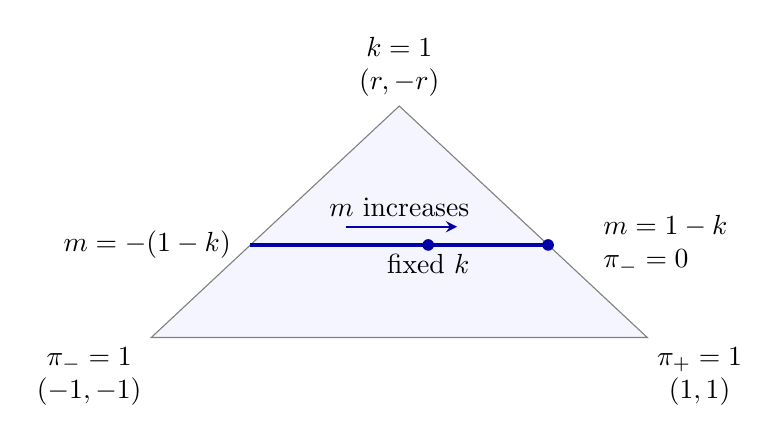
\begin{tikzpicture}[scale=1.05,>=stealth]
\coordinate (N) at (-3,0);
\coordinate (P) at (3,0);
\coordinate (C) at (0,2.8);
\fill[blue!4] (N)--(P)--(C)--cycle;
\draw[gray] (N)--(P)--(C)--cycle;
\node[below left,align=center] at (N) {$\pi_-=1$\\$(-1,-1)$};
\node[below right,align=center] at (P) {$\pi_+=1$\\$(1,1)$};
\node[above,align=center] at (C) {$k=1$\\$(r,-r)$};
\draw[very thick,blue!65!black] (-1.8,1.12)--(1.8,1.12);
\draw[->,thick,blue!65!black] (-.65,1.34)--(.7,1.34);
\node[above] at (0,1.34) {$m$ increases};
\fill[blue!65!black] (.35,1.12) circle (2pt);
\node[below] at (.35,1.12) {fixed $k$};
\fill[blue!65!black] (1.8,1.12) circle (2pt);
\node[right,align=left] at (2.35,1.12) {$m=1-k$\\$\pi_-=0$};
\node[left] at (-1.92,1.12) {$m=-(1-k)$};
\end{tikzpicture}

\caption{Mixture weights for a fixed reflected core $(r,-r)$.
The horizontal segment keeps its mass $k$ fixed, so the separation
$\delta=kr$, entropy $e=kH(r)$, and joining cost $\delta V(r)$ stay fixed.
Moving right increases the mean $m=\pi_+-\pi_-$ until the negative
common output disappears. Theorem~\ref{upgrade:joining} compares the
low-information demand with this endpoint. The triangle is schematic;
its points represent probability weights, not channel values.}
\label{fig:reflected-core}
\end{figure}

Figure~\ref{fig:reflected-core} displays the motion within the reflected
geometry. The path preserves the optimizer's cost and its average
entropy; the original law's individual entropies are retained separately
when applying the local production inequalities.
